\documentclass{article} % Defines the document class, article is commonly used
\usepackage[shortlabels]{enumitem}
\usepackage{amsmath}    % Allows for more advanced math formatting
\usepackage{amssymb}    % Provides additional mathematical symbols
\usepackage{amsthm}     % \qed
\usepackage{graphicx}   % image
\usepackage{float}      % image placement
\usepackage{siunitx}
\usepackage{hyperref}
\hypersetup{
    colorlinks=true,       % false: boxed links; true: colored links
    linkcolor=black,       % color of internal links
}
\usepackage[margin=1.5in]{geometry}

\begin{document}

\title{EEC133 Pre-Lab 1: Dipole Antennas and Noise}
\author{Tao Wang}
\date{\today}

\maketitle
\tableofcontents

\section*{Part 1: Dipole Antenna Design}
\addcontentsline{toc}{section}{Part 1: Dipole Antenna Design}
\begin{itemize}
    \item \textbf{Operating frequency:} 1.5 GHz
    \item \textbf{Length:} short dipole ($l \leq \frac{\lambda}{10}$)
    \item \textbf{Wire radius:} 0.5mm
    \item \textbf{Input impedance:} no requirement
\end{itemize}

\subsection*{Questions:}
\begin{enumerate}
    \item $l = 20$ mm

          We can find the wavelength $\lambda$ by $\lambda = \frac{c}{f} = \frac{\SI{3e8}{\meter\per\second}}{\SI{1.5e9}{\hertz}} = \SI{0.2}{m}$.

          The length of the dipole antenna is $l \leq  \frac{\lambda}{10} = \SI{20}{mm}$.

          Since the radiated power depends quadratically on $l$, the maximum $l$ gives the maximum radiated power.
    \item
          $$R_{rad} = 20 \pi^2 \left(\frac{l}{\lambda}\right)^2 = (20 \pi^2)\left(\frac{0.02}{0.2}\right)^2 = \SI{1.97}{\Omega}$$
          $$D_0 = 1.5$$
          $$F(\theta, \phi) = \sin^2(\theta)$$
          $$\text{HPBW} = \theta_2 - \theta_1 = 0.785-(-0.785) = 1.57$$
          $$\text{Far Field Requirement}: kr >> 1 \implies r >> \frac{\lambda}{2\pi} = \SI{0.03}{m}$$
    \item The normalized radiation intensity is radiation intensity of all direction normalized by the maximum radiation intensity.
          \begin{figure}[H]
              \centering
              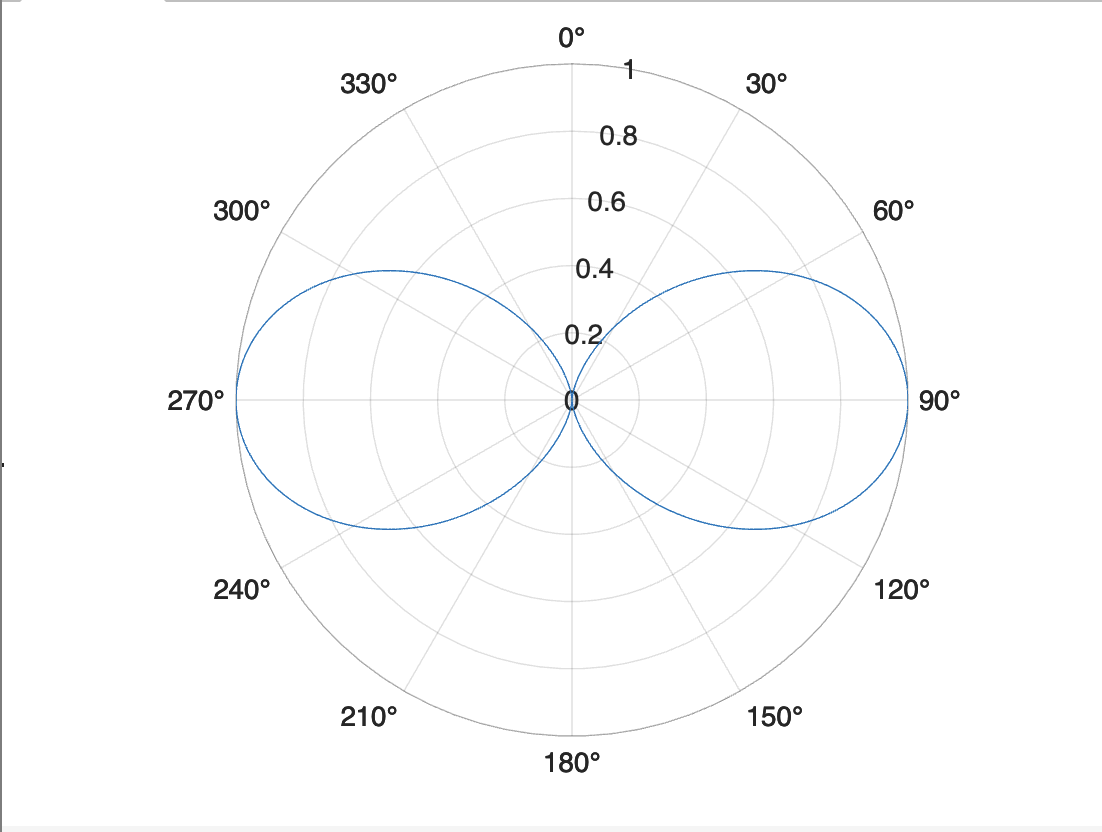
\includegraphics[width=0.5\textwidth]{./image/figure1.png}
              \caption{Normalized Radiation Intensity of the Dipole Antenna}
          \end{figure}
    \item HFSS Simulation
          \begin{enumerate}[(a)]
              \item Dipole Antenna Model
                    \begin{figure}[H]
                        \centering
                        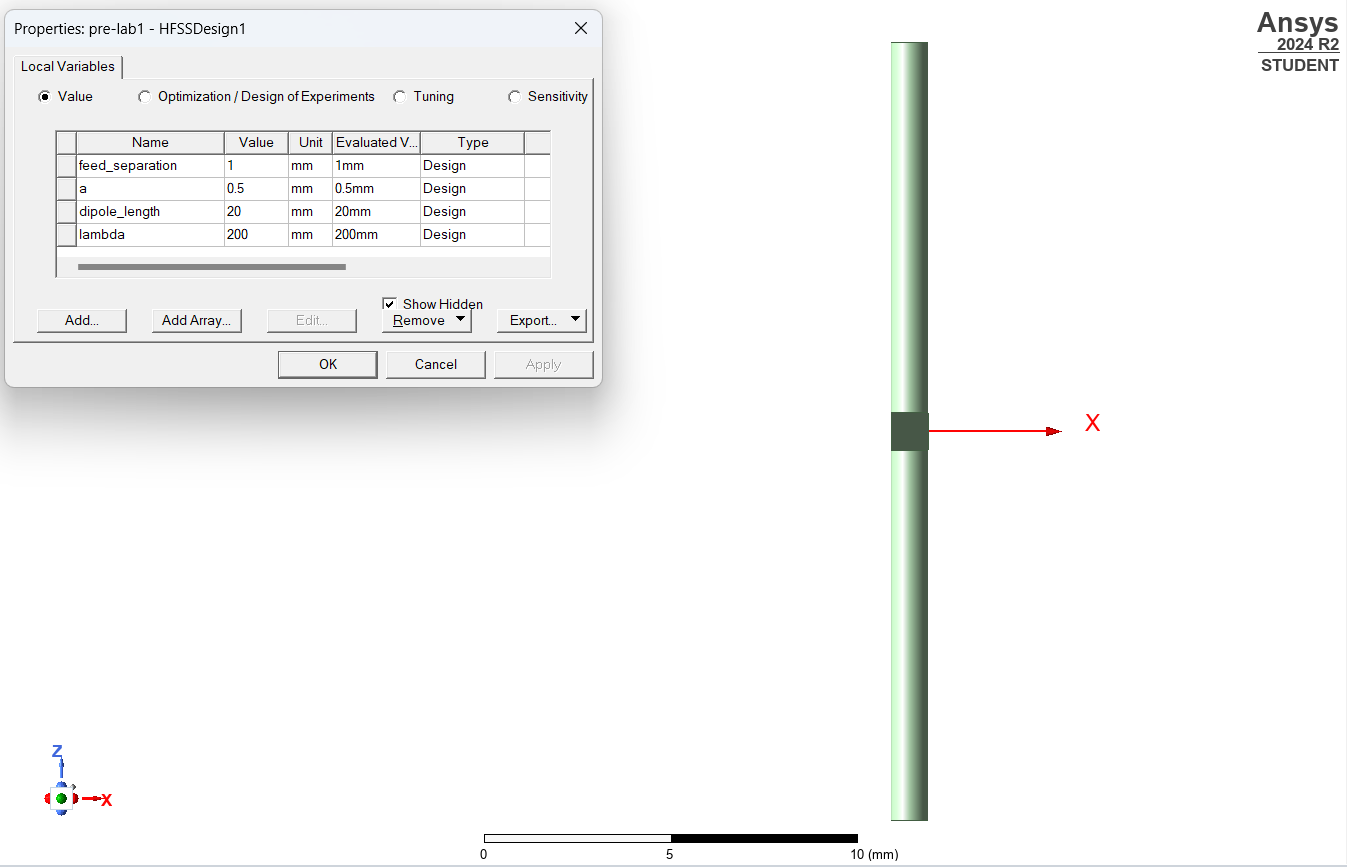
\includegraphics[width=0.7\textwidth]{./image/figure2.png}
                        \caption{Dipole Antenna Model}
                    \end{figure}
              \item S-Parameter
                    The S-Parameter frequency sweep plot shows that as the frequency increases, less of the input wave is reflected back.
                    \begin{figure}[H]
                        \centering
                        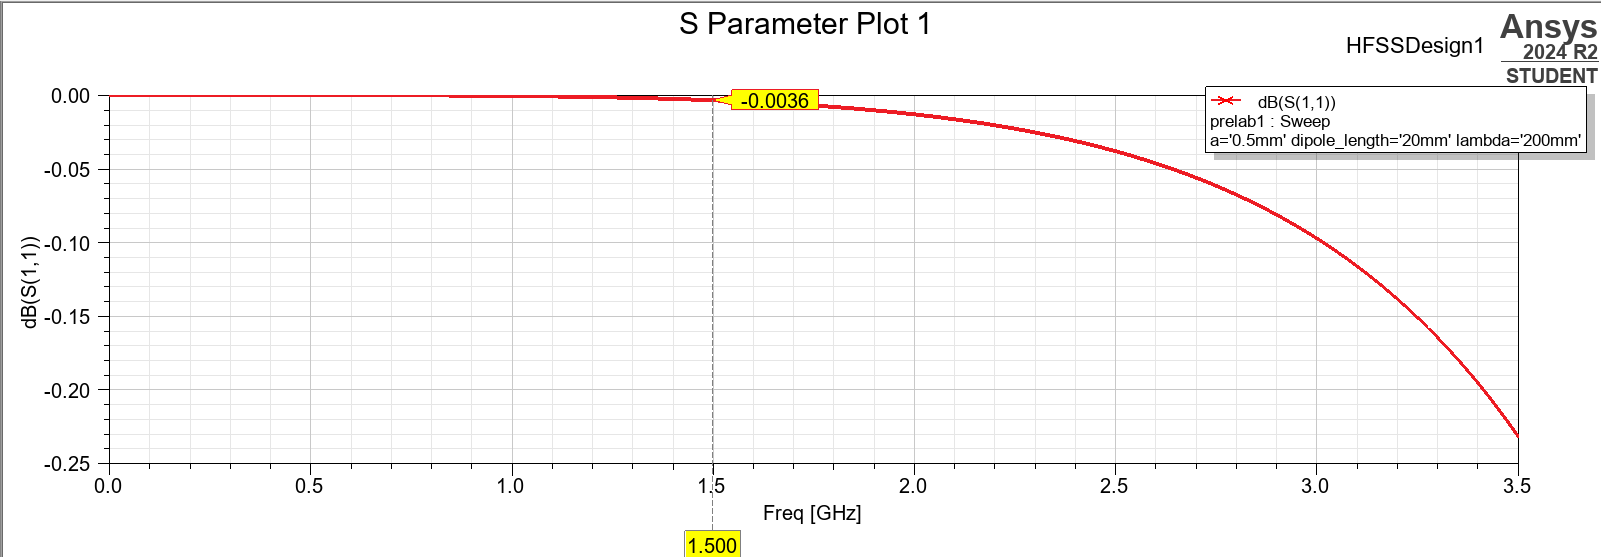
\includegraphics[width=0.7\textwidth]{./image/figure3.png}
                        \caption{S-Parameter Frequency Sweep}
                    \end{figure}
              \item 3D Directivity Pattern
                    \begin{figure}[H]
                        \centering
                        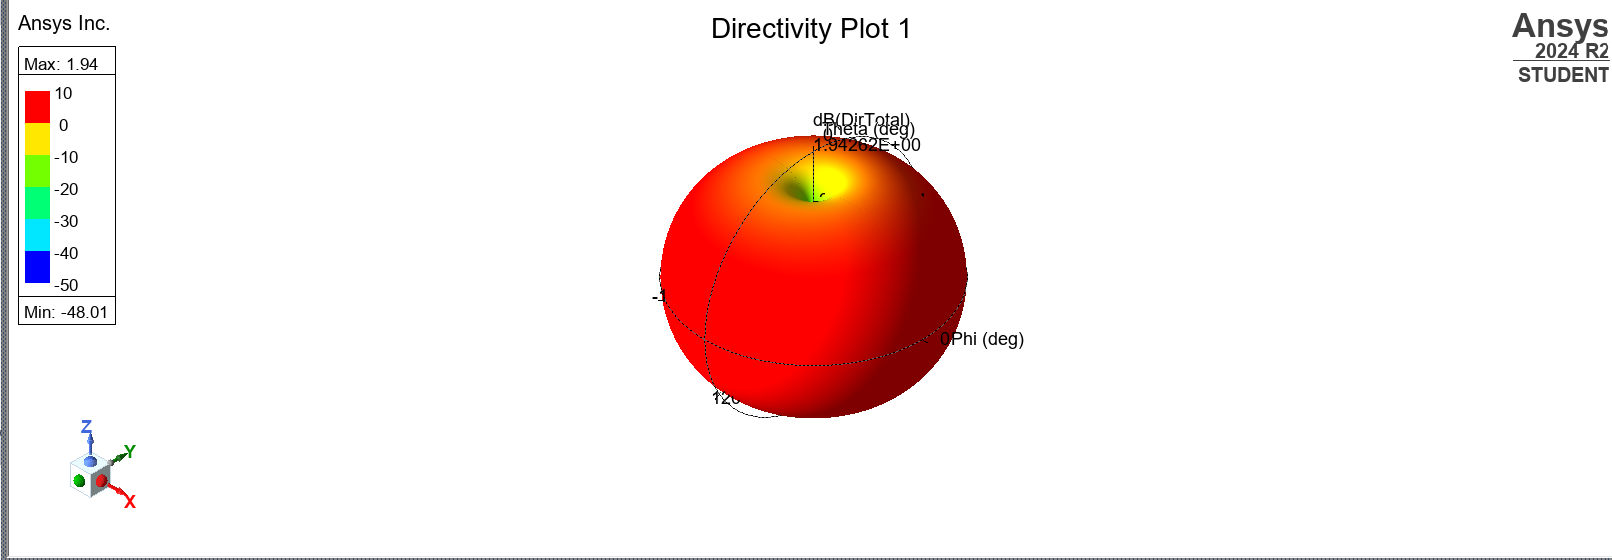
\includegraphics[width=1\textwidth]{./image/figure8.png}
                        \caption{3D Directivity Pattern}
                    \end{figure}
              \item Input impedance
                    $$Z_{in} = 1.81 -j 658.82 $$
                    The real part of the z parameter is less than the radiation resistance calculated in (2). The reactance make sense because the dipole antenna is geometrically similar to a capacitor. As a result, it has high reactance at low frequency, and low reactance at high frequency.
                    \begin{figure}[H]
                        \centering
                        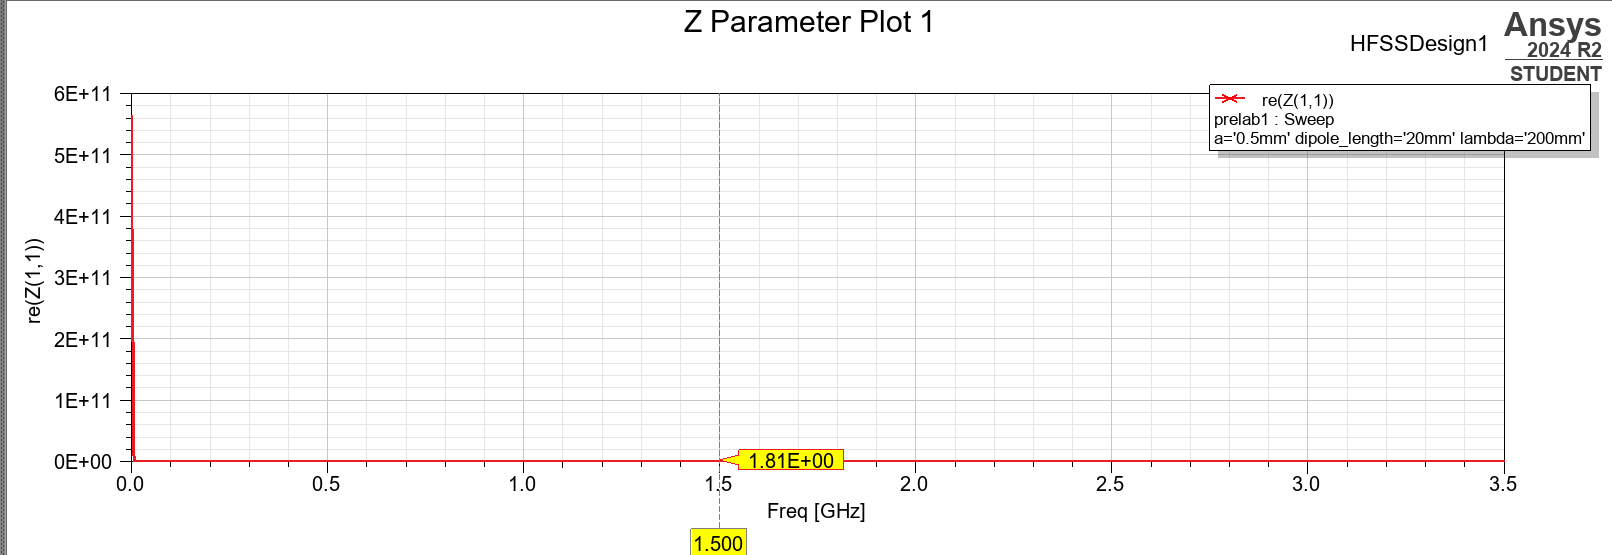
\includegraphics[width=0.7\textwidth]{./image/figure4.png}
                        \caption{$re(Z(1,1)$)}
                    \end{figure}
                    \begin{figure}[H]
                        \centering
                        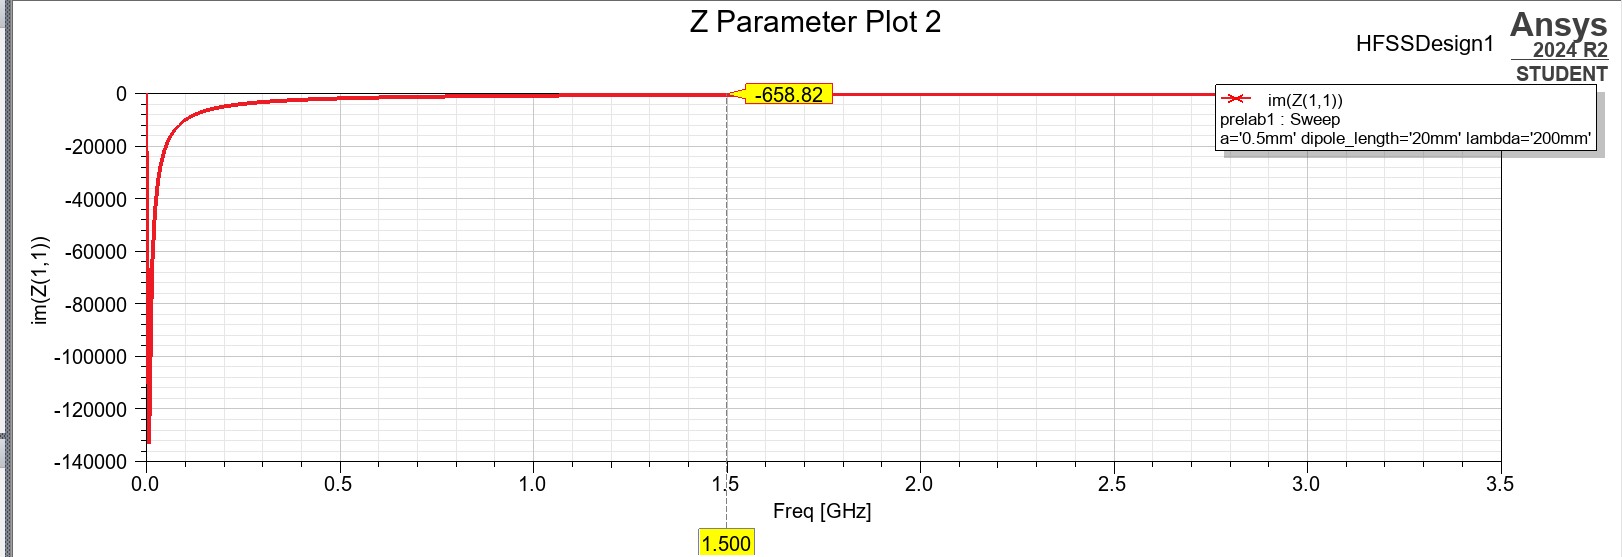
\includegraphics[width=0.7\textwidth]{./image/figure5.png}
                        \caption{$im(Z(1,1)$)}
                    \end{figure}
              \item The Electric Field
                    \begin{figure}[H]
                        \centering
                        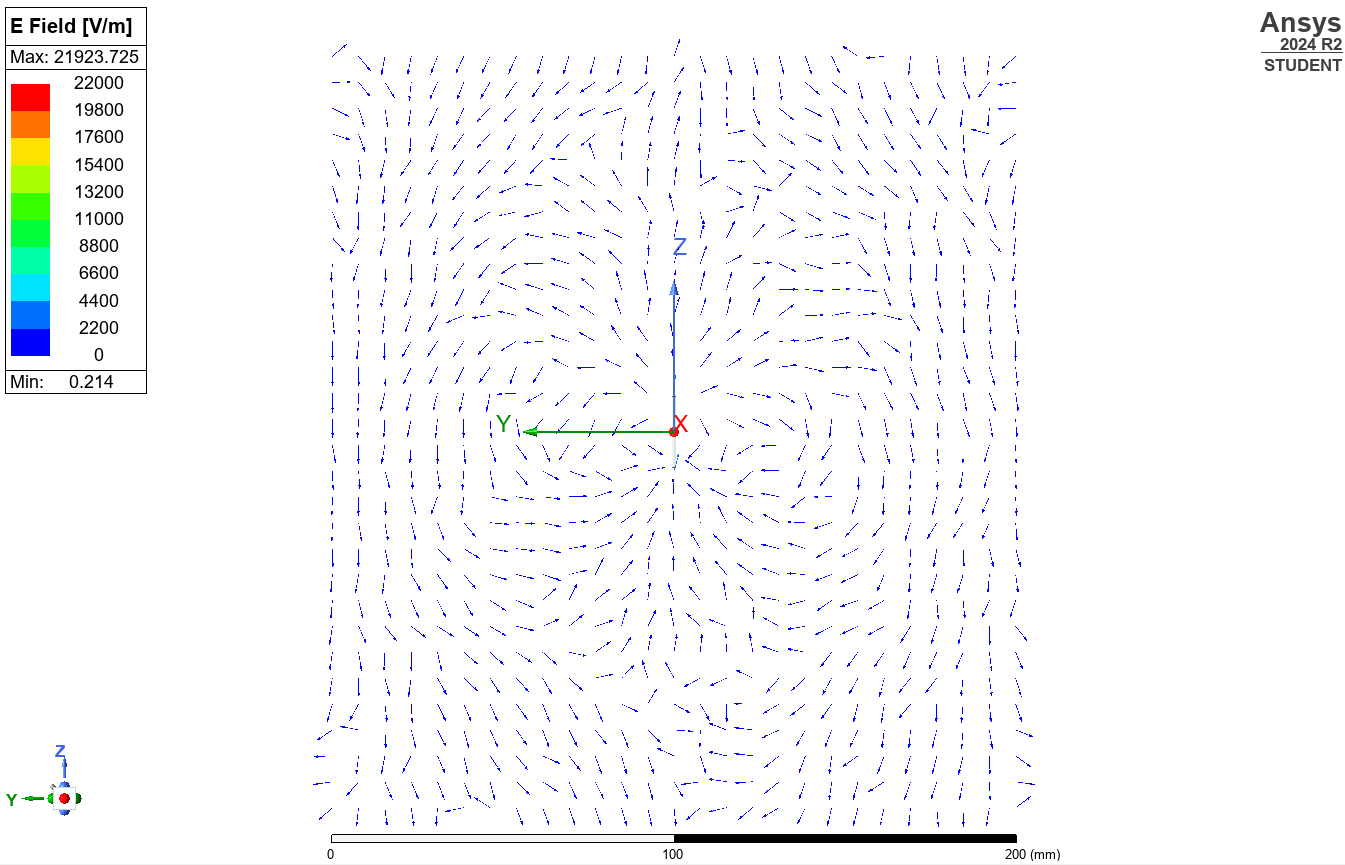
\includegraphics[width=0.5\textwidth]{./image/figure6.png}
                        \caption{$\vec{E}$ Field}
                    \end{figure}
              \item The Magnetic Field
                    \begin{figure}[H]
                        \centering
                        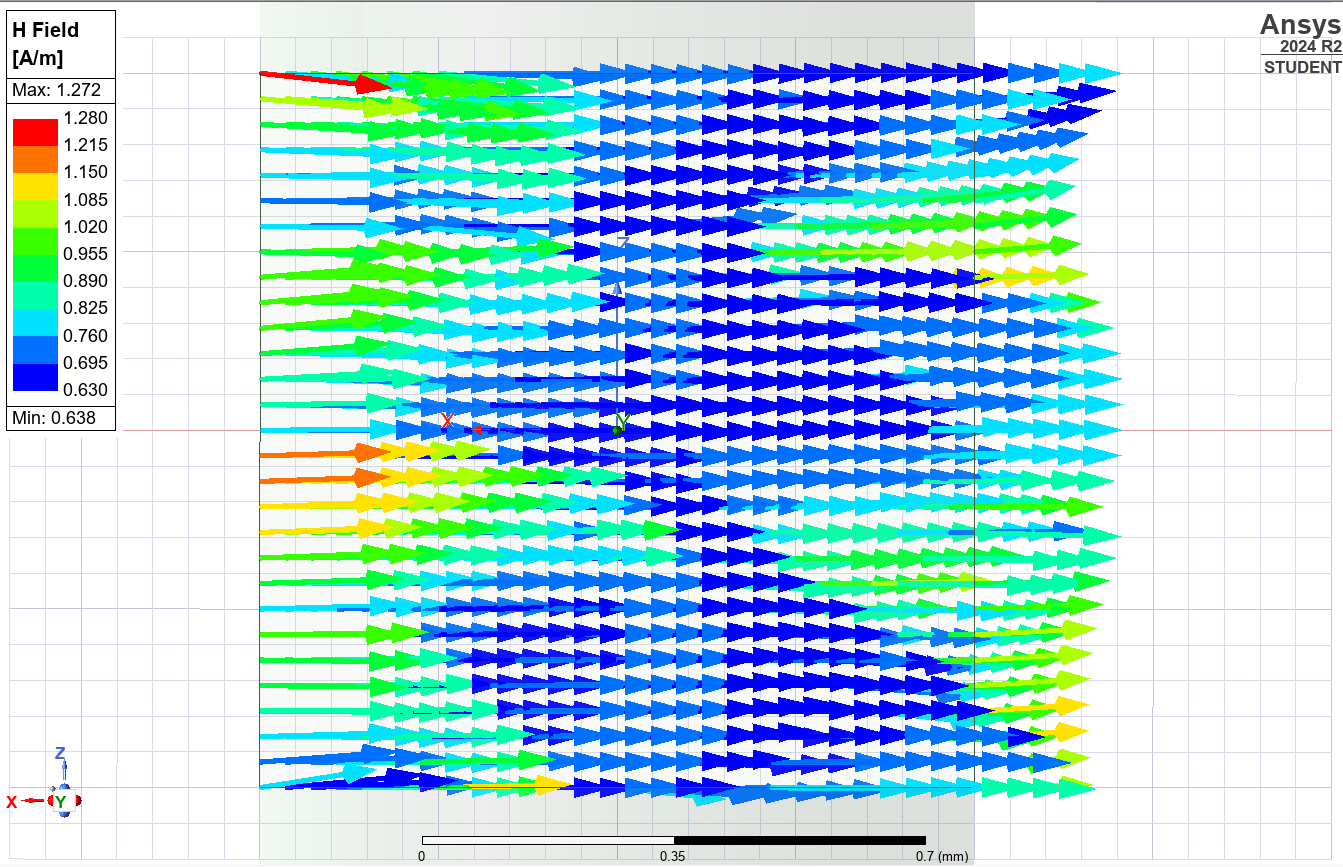
\includegraphics[width=0.5\textwidth]{./image/figure7.png}
                        \caption{$\vec{H}$ Field}
                    \end{figure}
              \item The antenna is not a good transmitter because $R_{rad}$ is small, so it's hard to match its impedance and reduce reflected power.
          \end{enumerate}
\end{enumerate}

\pagebreak
\section*{Part 2: Basic Noise Calculations}
\addcontentsline{toc}{section}{Part 2: Basic Noise Calculations}
\begin{enumerate}
    \item Approximate Noise Level = $\SI{-102}{dBm}$
    \item
          $$P_n = \left(1.38 \times 10^{-23} \si{\frac{\joule}{\kelvin}}\right)(298.15 \si{\kelvin})(1 \times 10^6 \si{\hertz}) = 4.1 \times 10^{-15} \si{\watt}$$
          $$\text{Expected Noise Level = }10 \log\left(\frac{P_{in}}{10^{-3}}\right) = -113.9 \text{ } \si{ dBm}$$
    \item
          $$P = (1 \text{ }\si{mW})\left(10^\frac{-102 \si{dBm}}{10 \si{dBm}}\right) = 6.3 \times 10^{-14} \si{\watt}$$
    \item In both cases, spikes could be observed in the 2.4 - 2.4 GHz range. However, the spikes are bigger when the antenna is attached. These spikes are from the bluetooth signals.
    \item Yes, the electric field from the bluetooth wave induces current oscillations in the transmission line. The time-varying current carries AC power, which is plotted on the network analyzer. When the transmission line is opened at the end, the impedance is purely reactive, thus no power is dissipated. Therefore, no power is detected in the analyzer except those from the resistor's thermal noise. As a result, we only see a weak signal because it's only caused by the thermal noise.
\end{enumerate}

\end{document}
